\documentclass{standalone}
\usepackage{tikz}
\usetikzlibrary{patterns, positioning}
\usepackage[sfdefault]{ClearSans} %% option 'sfdefault' activates Clear Sans as the default text font
\usepackage[T1]{fontenc}

\begin{document}
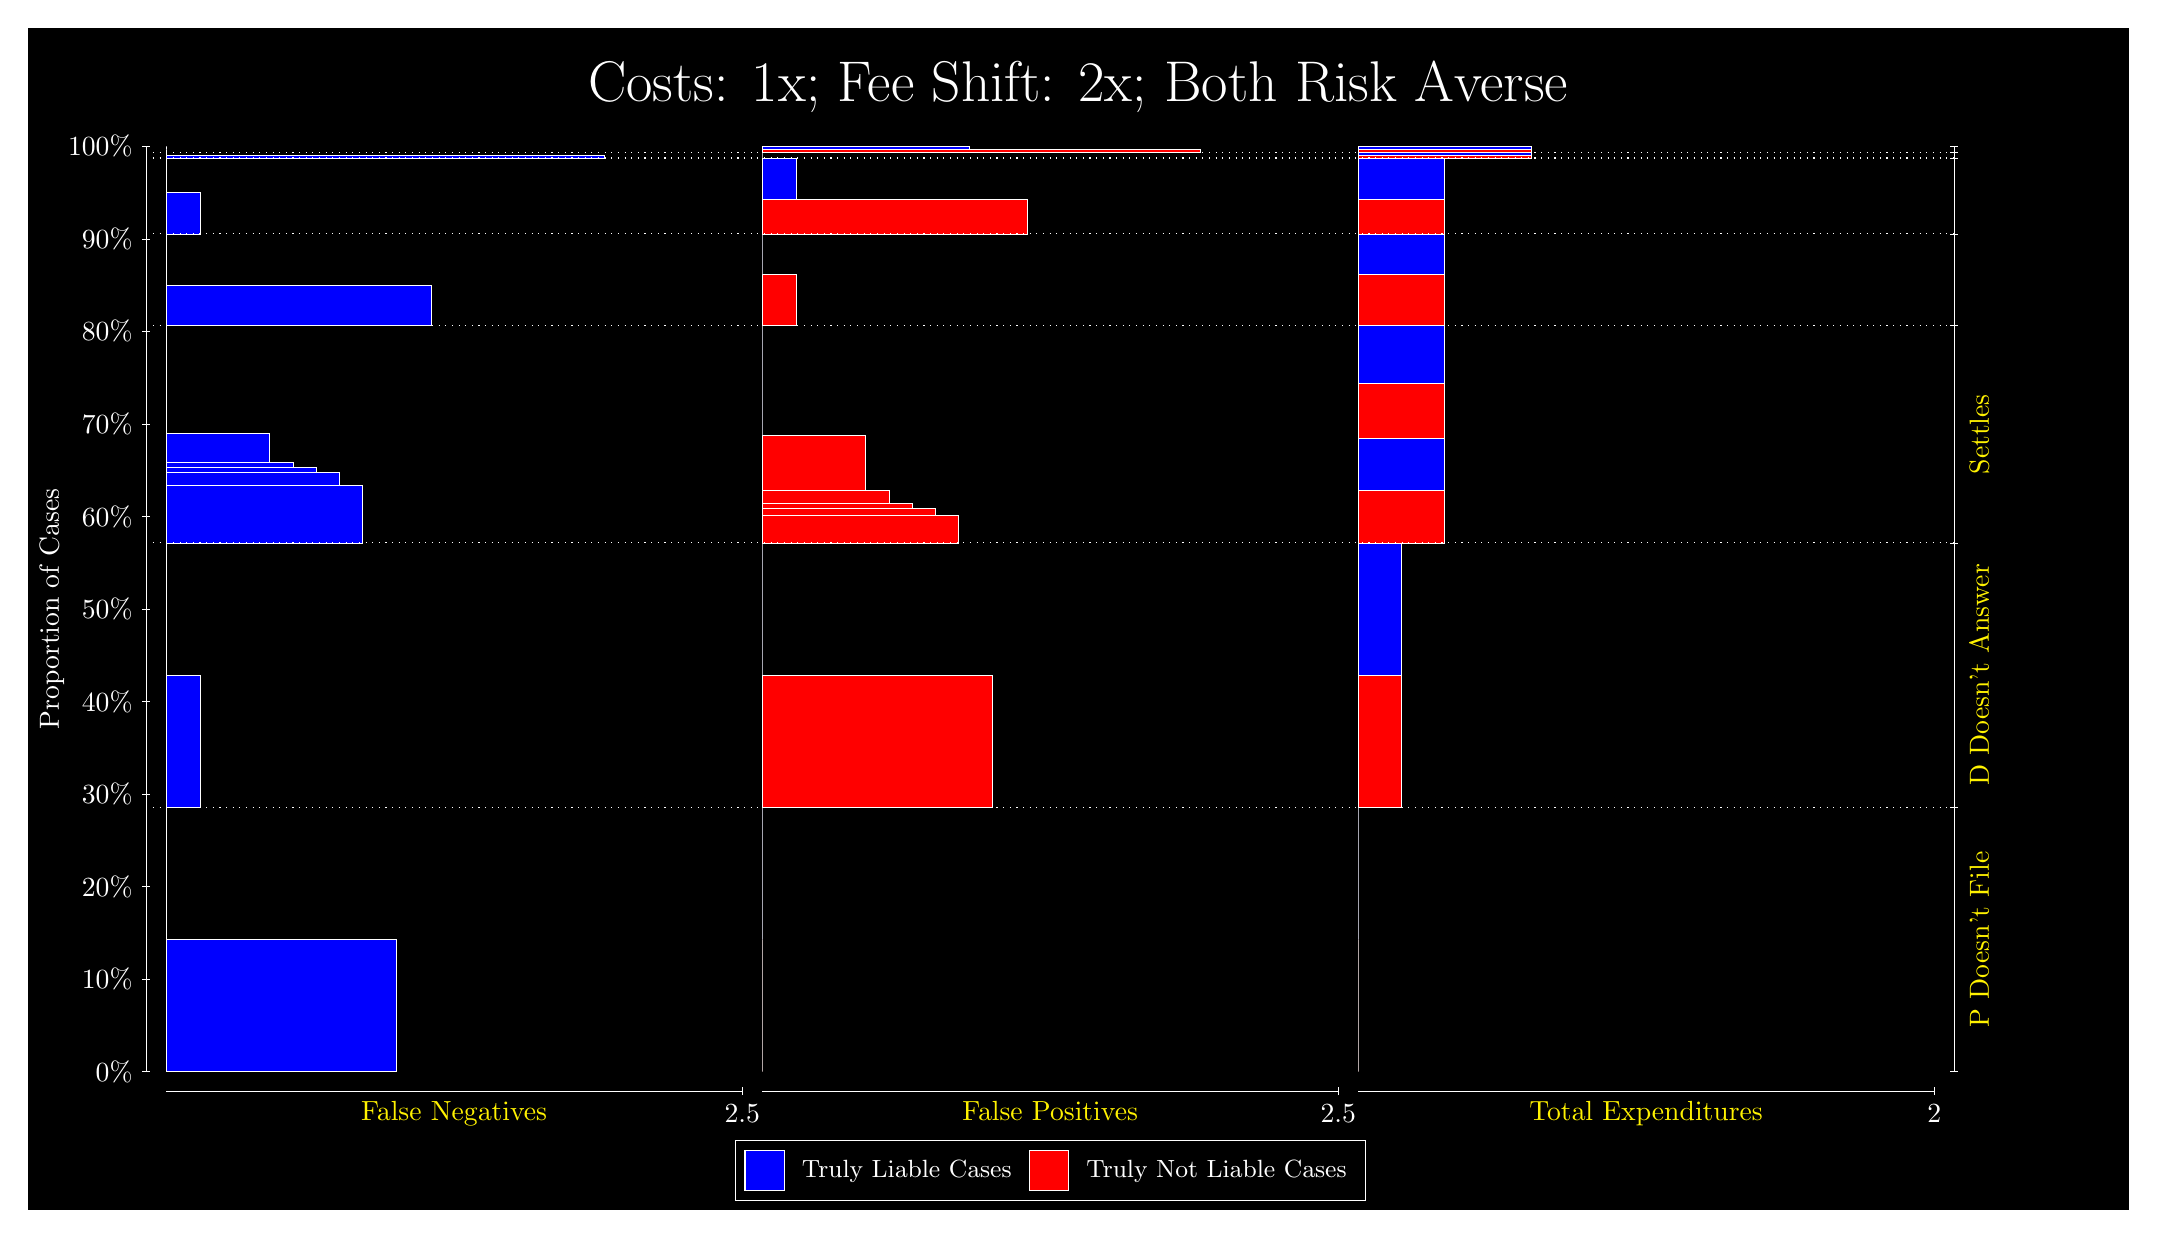
\begin{tikzpicture}
\draw[fill=black] (0,0) rectangle (26.667,15);
\draw[text=white] (0,13.5) rectangle (26.667,15) node[midway] {\huge Costs: 1x; Fee Shift: 2x; Both Risk Averse};
\draw[white, very thin] (1.5,1.75) -- (1.5,13.5);
\node[rotate=90, text=white, anchor=center] at (0.3, 7.625) {Proportion of Cases};
\draw[white, very thin] (1.45,1.75) -- (1.55,1.75);
\node[text=white, anchor=east] at (1.45, 1.75) {0\%};
\draw[white, very thin] (1.45,2.925) -- (1.55,2.925);
\node[text=white, anchor=east] at (1.45, 2.925) {10\%};
\draw[white, very thin] (1.45,4.1) -- (1.55,4.1);
\node[text=white, anchor=east] at (1.45, 4.1) {20\%};
\draw[white, very thin] (1.45,5.275) -- (1.55,5.275);
\node[text=white, anchor=east] at (1.45, 5.275) {30\%};
\draw[white, very thin] (1.45,6.45) -- (1.55,6.45);
\node[text=white, anchor=east] at (1.45, 6.45) {40\%};
\draw[white, very thin] (1.45,7.625) -- (1.55,7.625);
\node[text=white, anchor=east] at (1.45, 7.625) {50\%};
\draw[white, very thin] (1.45,8.8) -- (1.55,8.8);
\node[text=white, anchor=east] at (1.45, 8.8) {60\%};
\draw[white, very thin] (1.45,9.975) -- (1.55,9.975);
\node[text=white, anchor=east] at (1.45, 9.975) {70\%};
\draw[white, very thin] (1.45,11.15) -- (1.55,11.15);
\node[text=white, anchor=east] at (1.45, 11.15) {80\%};
\draw[white, very thin] (1.45,12.325) -- (1.55,12.325);
\node[text=white, anchor=east] at (1.45, 12.325) {90\%};
\draw[white, very thin] (1.45,13.5) -- (1.55,13.5);
\node[text=white, anchor=east] at (1.45, 13.5) {100\%};

\draw[white, very thin] (24.457,1.75) -- (24.457,13.5);
\draw[white, very thin] (24.407,1.75) -- (24.507,1.75);
\node[anchor=west] at (24.407, 1.75) {};
\draw[white, very thin] (24.407,5.1071) -- (24.507,5.1071);
\node[anchor=west] at (24.407, 5.1071) {};
\draw[white, very thin] (24.407,8.4643) -- (24.507,8.4643);
\node[anchor=west] at (24.407, 8.4643) {};
\draw[white, very thin] (24.407,11.223) -- (24.507,11.223);
\node[anchor=west] at (24.407, 11.223) {};
\draw[white, very thin] (24.407,12.389) -- (24.507,12.389);
\node[anchor=west] at (24.407, 12.389) {};
\draw[white, very thin] (24.407,13.352) -- (24.507,13.352);
\node[anchor=west] at (24.407, 13.352) {};
\draw[white, very thin] (24.407,13.426) -- (24.507,13.426);
\node[anchor=west] at (24.407, 13.426) {};
\draw[white, very thin] (24.407,13.5) -- (24.507,13.5);
\node[anchor=west] at (24.407, 13.5) {};

\draw[white, very thin, fill=blue] (1.75,1.75) rectangle (4.6775,3.4286);
\draw[white, very thin, fill=red] (1.75,3.4286) rectangle (1.75,5.1071);
\draw[white, very thin, fill=blue] (1.75,5.1071) rectangle (2.1891,6.7857);
\draw[white, very thin, fill=red] (1.75,6.7857) rectangle (1.75,8.4643);
\draw[white, very thin, fill=blue] (1.75,8.4643) rectangle (4.2384,9.1944);
\draw[white, very thin, fill=blue] (1.75,9.1944) rectangle (3.9457,9.3575);
\draw[white, very thin, fill=blue] (1.75,9.3575) rectangle (3.6529,9.4191);
\draw[white, very thin, fill=blue] (1.75,9.4191) rectangle (3.3602,9.4929);
\draw[white, very thin, fill=blue] (1.75,9.4929) rectangle (3.0674,9.8613);
\draw[white, very thin, fill=red] (1.75,9.8613) rectangle (1.75,11.223);
\draw[white, very thin, fill=blue] (1.75,11.223) rectangle (5.1167,11.74);
\draw[white, very thin, fill=red] (1.75,11.74) rectangle (1.75,12.389);
\draw[white, very thin, fill=blue] (1.75,12.389) rectangle (2.1891,12.919);
\draw[white, very thin, fill=red] (1.75,12.919) rectangle (1.75,13.352);
\draw[white, very thin, fill=blue] (1.75,13.352) rectangle (7.3123,13.386);
\draw[white, very thin, fill=red] (1.75,13.386) rectangle (1.75,13.426);
\draw[white, very thin, fill=red] (1.75,13.426) rectangle (1.75,13.46);
\draw[white, very thin, fill=blue] (1.75,13.46) rectangle (1.75,13.5);
\draw[white, very thin, fill=red] (9.3189,1.75) rectangle (9.3189,3.4286);
\draw[white, very thin, fill=blue] (9.3189,3.4286) rectangle (9.3189,5.1071);
\draw[white, very thin, fill=red] (9.3189,5.1071) rectangle (12.246,6.7857);
\draw[white, very thin, fill=blue] (9.3189,6.7857) rectangle (9.3189,8.4643);
\draw[white, very thin, fill=red] (9.3189,8.4643) rectangle (11.807,8.8107);
\draw[white, very thin, fill=red] (9.3189,8.8107) rectangle (11.515,8.8984);
\draw[white, very thin, fill=red] (9.3189,8.8984) rectangle (11.222,8.9686);
\draw[white, very thin, fill=red] (9.3189,8.9686) rectangle (10.929,9.1266);
\draw[white, very thin, fill=red] (9.3189,9.1266) rectangle (10.636,9.8262);
\draw[white, very thin, fill=blue] (9.3189,9.8262) rectangle (9.3189,11.223);
\draw[white, very thin, fill=red] (9.3189,11.223) rectangle (9.758,11.872);
\draw[white, very thin, fill=blue] (9.3189,11.872) rectangle (9.3189,12.389);
\draw[white, very thin, fill=red] (9.3189,12.389) rectangle (12.686,12.822);
\draw[white, very thin, fill=blue] (9.3189,12.822) rectangle (9.758,13.352);
\draw[white, very thin, fill=red] (9.3189,13.352) rectangle (9.3189,13.392);
\draw[white, very thin, fill=blue] (9.3189,13.392) rectangle (9.3189,13.426);
\draw[white, very thin, fill=red] (9.3189,13.426) rectangle (14.881,13.46);
\draw[white, very thin, fill=blue] (9.3189,13.46) rectangle (11.954,13.5);
\draw[white, very thin, fill=red] (16.888,1.75) rectangle (16.888,3.4286);
\draw[white, very thin, fill=blue] (16.888,3.4286) rectangle (16.888,5.1071);
\draw[white, very thin, fill=red] (16.888,5.1071) rectangle (17.437,6.7857);
\draw[white, very thin, fill=blue] (16.888,6.7857) rectangle (17.437,8.4643);
\draw[white, very thin, fill=red] (16.888,8.4643) rectangle (17.986,9.1266);
\draw[white, very thin, fill=blue] (16.888,9.1266) rectangle (17.986,9.7936);
\draw[white, very thin, fill=red] (16.888,9.7936) rectangle (17.986,10.493);
\draw[white, very thin, fill=blue] (16.888,10.493) rectangle (17.986,11.223);
\draw[white, very thin, fill=red] (16.888,11.223) rectangle (17.986,11.872);
\draw[white, very thin, fill=blue] (16.888,11.872) rectangle (17.986,12.389);
\draw[white, very thin, fill=red] (16.888,12.389) rectangle (17.986,12.822);
\draw[white, very thin, fill=blue] (16.888,12.822) rectangle (17.986,13.352);
\draw[white, very thin, fill=red] (16.888,13.352) rectangle (19.083,13.392);
\draw[white, very thin, fill=blue] (16.888,13.392) rectangle (19.083,13.426);
\draw[white, very thin, fill=red] (16.888,13.426) rectangle (19.083,13.46);
\draw[white, very thin, fill=blue] (16.888,13.46) rectangle (19.083,13.5);
\draw[white, dotted] (1.5,5.1071) -- (24.457,5.1071);
\draw[white, dotted] (1.5,8.4643) -- (24.457,8.4643);
\draw[white, dotted] (1.5,11.223) -- (24.457,11.223);
\draw[white, dotted] (1.5,12.389) -- (24.457,12.389);
\draw[white, dotted] (1.5,13.352) -- (24.457,13.352);
\draw[white, dotted] (1.5,13.426) -- (24.457,13.426);
\draw[white, very thin] (1.75,1.5) -- (9.0689,1.5);
\node[text=yellow, anchor=north] at (5.4094, 1.5) {False Negatives};
\draw[white, very thin] (9.0689,1.45) -- (9.0689,1.55);
\node[text=white, anchor=north] at (9.0689, 1.45) {2.5};

\draw[white, very thin] (9.3189,1.5) -- (16.638,1.5);
\node[text=yellow, anchor=north] at (12.978, 1.5) {False Positives};
\draw[white, very thin] (16.638,1.45) -- (16.638,1.55);
\node[text=white, anchor=north] at (16.638, 1.45) {2.5};

\draw[white, very thin] (16.888,1.5) -- (24.207,1.5);
\node[text=yellow, anchor=north] at (20.547, 1.5) {Total Expenditures};
\draw[white, very thin] (24.207,1.45) -- (24.207,1.55);
\node[text=white, anchor=north] at (24.207, 1.45) {2};

\node[text=yellow, centered, rotate=90] at (24.777, 3.4286) {P Doesn't File};
\node[text=yellow, centered, rotate=90] at (24.777, 6.7857) {D Doesn't Answer};
\node[text=yellow, centered, rotate=90] at (24.777, 9.8438) {Settles};





\draw (12.978300999999998,1.5) node[draw=none] (baseCoordinate) {};
\begin{scope}[align=center]
        \matrix[scale=0.5, draw=white, below=0.5cm of baseCoordinate, nodes={draw}, column sep=0.1cm]{
            \node[rectangle, draw, minimum width=0.5cm, minimum height=0.5cm, fill=blue] {}; &
            \node[draw=none, font=\small, text=white] (B) {Truly Liable Cases}; &
            \node[rectangle, draw, minimum width=0.5cm, minimum height=0.5cm, fill=red] {}; &
            \node[draw=none, font=\small, text=white] (B) {Truly Not Liable Cases}; \\
            };
\end{scope}

\end{tikzpicture}
\end{document}